\documentclass[../main.tex]{subfiles}
\begin{document}
\chapter{Results}

\section{Covariance or correlation matrix}
Table \ref{tab:correlation_matrix_dataset} shows the correlation between the variables of the dataset and their standard deviations. A few cases have a high correlation (e.g., fat and sodium; ash and carbohydrates; ash and proteins; ash and sodium). Regarding the standard deviations, there are important differences between them ($\sigma_{carb}=18.029722$, $\sigma_{sodium}=0.370358$).
\begin{table}[H]
\resizebox{\textwidth}{!}{%
\begin{tabular}{|l|c|c|c|c|c|c|c|}
                & \multicolumn{1}{l}{\textbf{ash}} & \multicolumn{1}{l}{\textbf{cal}} & \multicolumn{1}{l}{\textbf{carb}} & \multicolumn{1}{l}{\textbf{fat}} & \multicolumn{1}{l}{\textbf{mois}} & \multicolumn{1}{l}{\textbf{prot}} & \multicolumn{1}{l}{\textbf{sodium}} \\
\textbf{ash}    & 1                                &                                  &                                   &                                  &                                   &                                   &                                     \\ \hline
\textbf{cal}    & 0.326468                         & 1                                &                                   &                                  &                                   &                                   &                                     \\ \hline
\textbf{carb}   & -0.898988                        & -0.023485                        & 1                                 &                                  &                                   &                                   &                                     \\ \hline
\textbf{fat}    & 0.791634                         & 0.764567                         & -0.640238                         & 1                                &                                   &                                   &                                     \\ \hline
\textbf{mois}   & 0.265556                         & -0.764441                        & -0.591802                         & -0.171318                        & 1                                 &                                   &                                     \\ \hline
\textbf{prot}   & 0.823844                         & 0.070258                         & -0.853542                         & 0.498002                         & 0.360248                          & 1                                 &                                     \\ \hline

\textbf{sodium} & 0.808122                         & 0.671958                         & -0.620176                         & 0.933325                         & -0.102279                         & 0.429130                          & 1      \\ \hline \hline
\textbf{Standard Deviations} & 1.269724 & 0.620034 & 18.029722 & 8.975658 & 9.552987 & 6.434392 & 0.370358 \\ \hline
\end{tabular}%
}
\caption{Correlation matrix between variables of the dataset and their standard deviation.}
\label{tab:correlation_matrix_dataset}
\end{table}

\section{Number of Principal Component}
From the scree plot in figure \ref{fig:scree_plot} the elbow is clearly visible at PC number three. Also, the cumulative variance (in table \ref{tab:cumulative_variance}) reinforces this choice.
\begin{figure}[H]
    \centering
    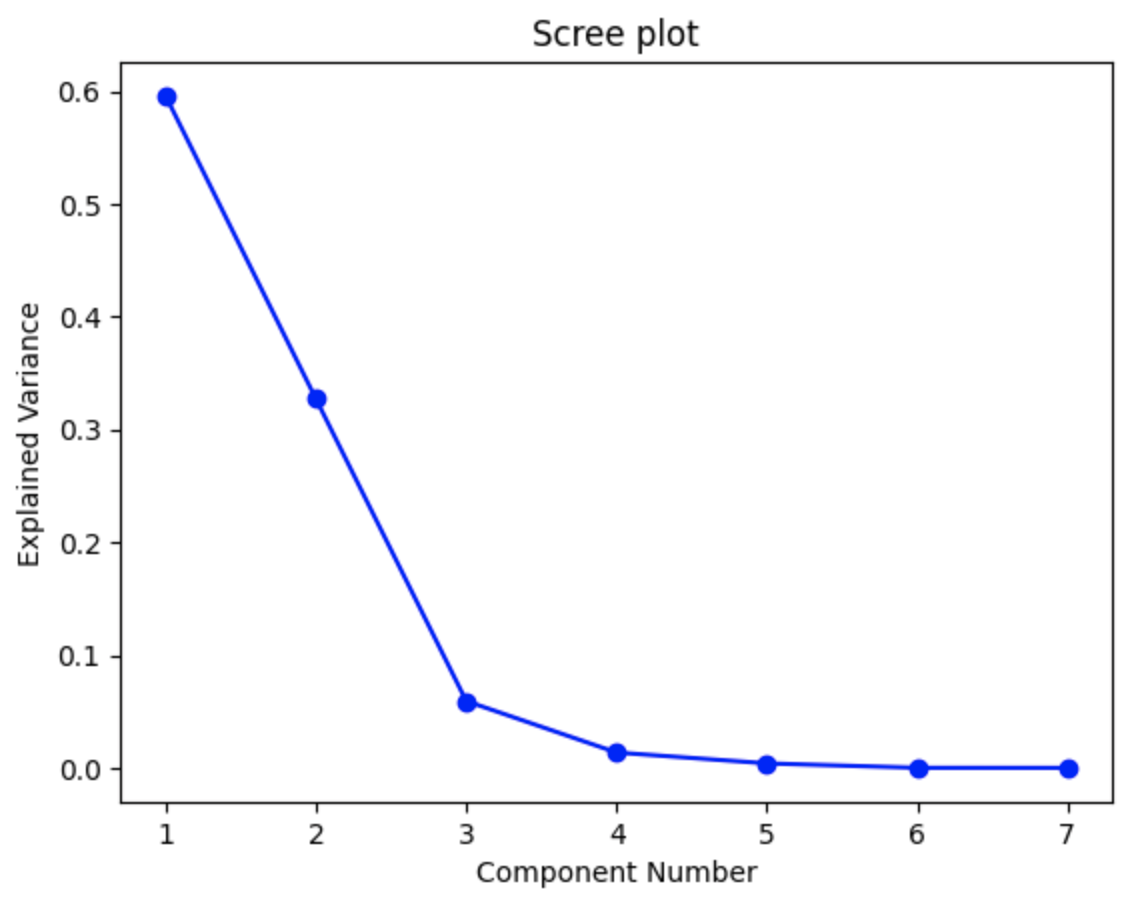
\includegraphics[width=\columnwidth]{img/screePlot.png}
    \caption{Scree plot}
    \label{fig:scree_plot}
\end{figure}

\begin{table}[H]
\resizebox{\textwidth}{!}{%
\begin{tabular}{|c|c|c|c|c|c|c|}
\hline
\textbf{PC1} & \textbf{PC2} & \textbf{PC3} & \textbf{PC4} & \textbf{PC5} & \textbf{PC6} & \textbf{PC7} \\ \hline
0.59596884 & 0.92317704 & 0.98240023 & 0.99599655 & 0.99995041 & 0.99999864 & 1                \\ \hline
\end{tabular}%
}
\caption{Cumulative variances}
\label{tab:cumulative_variance}
\end{table}

\section{Understand the results}
Figure \ref{fig:correlation_matrix} shows the correlation matrix between the PCs and the features of the dataset. It shows a high correlation between:
\begin{itemize}
    \item PC1 with ash, carbohydrates, fat, and sodium;
    \item PC2 with calories and moisture;
    \item PC3 with moisture, proteins, and sodium.
\end{itemize}
\begin{figure}[H]
    \centering
    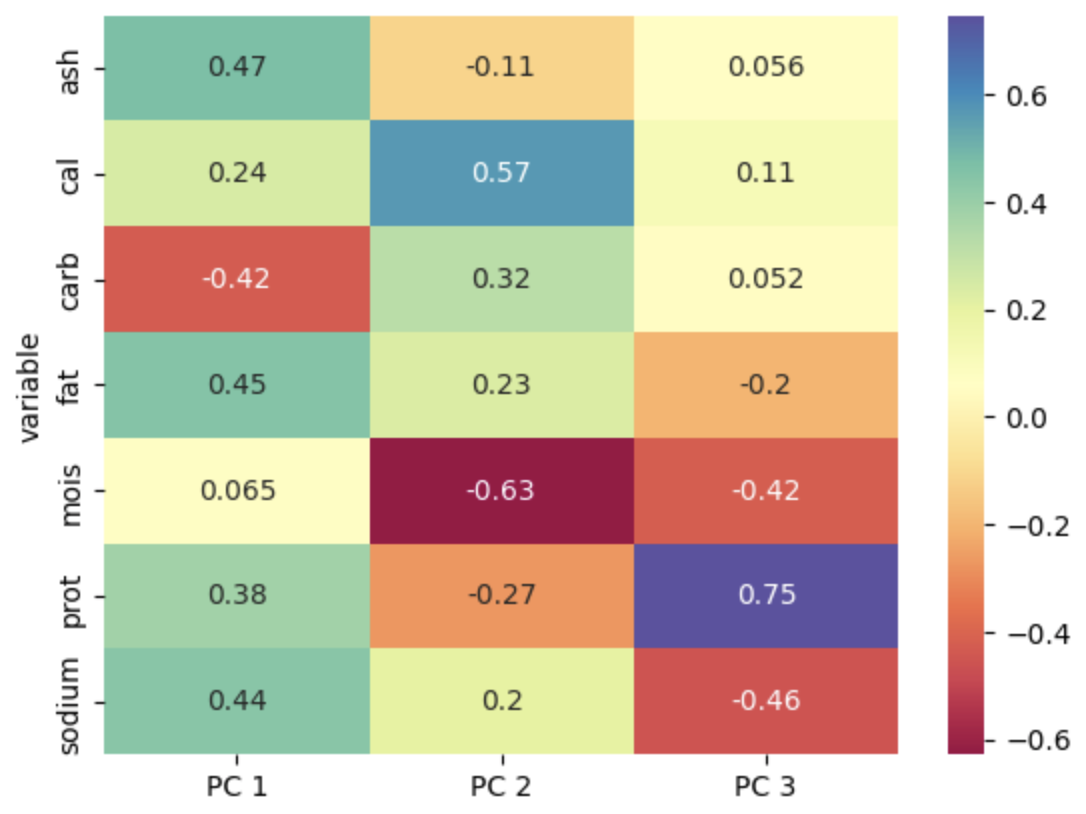
\includegraphics[width=\columnwidth]{img/correlationMatrix.png}
    \caption{Correlation matrix between PCs and dataset's feature}
    \label{fig:correlation_matrix}
\end{figure}

\section{Plot the Principal Components}
To visualize the results of PCA, a 3D scatter plot has been used. The result (figure \ref{fig:plot_pca}) shows in different colors the ten different brands in the dataset. Five groups can be easily recognized from the image:
\begin{itemize}
    \item red;
    \item blue;
    \item orange;
    \item yellow;
    \item others colors.
\end{itemize}
\begin{figure}[H]
    \centering
    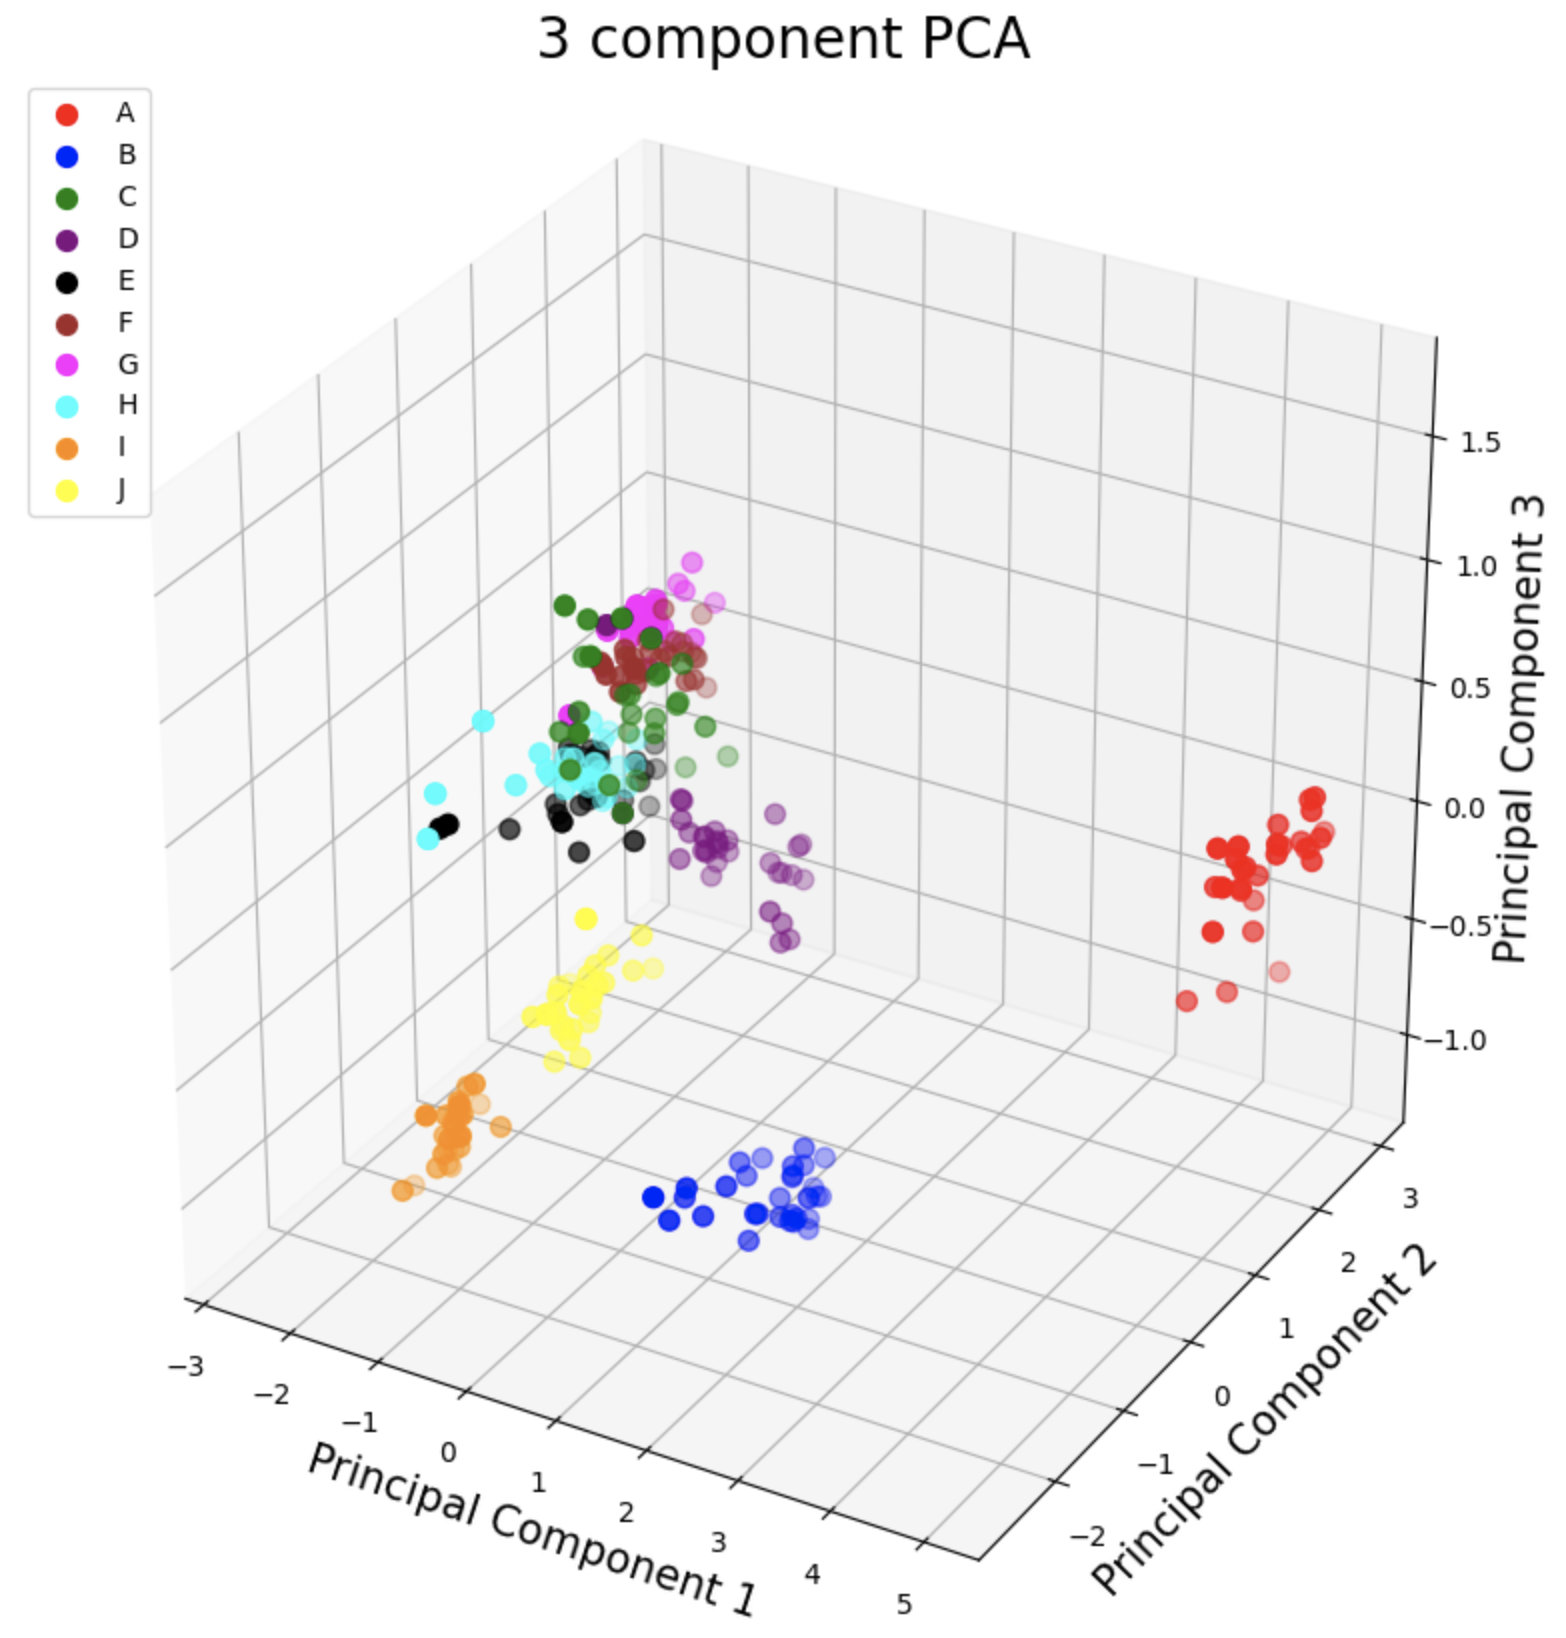
\includegraphics[width=\columnwidth]{img/plotPCA.png}
    \caption{3D Scatter plot of the first three PCs}
    \label{fig:plot_pca}
\end{figure}

\end{document}